\documentclass[12pt,a4paper]{article}

% Packages
\usepackage[utf8]{inputenc}
\usepackage[english]{babel}
\usepackage{amsmath}
\usepackage{graphicx}
\usepackage{cite}
\usepackage{hyperref}
\usepackage{geometry}
\geometry{margin=1in}
\usepackage{setspace}
\usepackage{wrapfig}
\onehalfspacing
\usepackage[protrusion=true,expansion=true]{microtype}
\usepackage{hyphenat}   % Better hyphenation control
\usepackage{booktabs}  % For better tables if you add any
\usepackage{lipsum}    % Remove this later, just for placeholder text
\sloppy  % Allows more flexibility in line breaking

\onehalfspacing

% Title and Author
\title{Agentic Framework for Biomarker Discovery from Electronic Health Records}
\author{Ofek Vilkerstone \\ 212712608}
\date{\today}

\begin{document}

\maketitle

\begin{abstract}
Composite biomarkers prove clinically powerful, yet their discovery remains slow and expert-driven. Machine learning offers automation, but lacks systematic comparison frameworks—and sophisticated methods target expensive measurements while accessible-data studies use simple analytics.

We present an agentic framework with interchangeable logic for automated biomarker discovery from routine Complete Blood Count measurements (\$10-30 versus \$100-1000 proteomics). The framework enables controlled comparison of random generation, genetic programming, and large language models across four immunological diseases.

Our contributions: (1) first systematic method comparison under identical conditions, (2) explicit testing of data-driven versus literature-guided feature selection, (3) sophisticated methods applied to universally accessible measurements, and (4) quantified interpretability-performance trade-offs. The modular architecture separates fixed pipelines from interchangeable generation logic, advancing both discovery science and clinical deployment.
\end{abstract}
\newpage
\setcounter{tocdepth}{2} 
\tableofcontents
\newpage

\section{Introduction}

Every year, millions of patients receive Complete Blood Count (CBC) tests—one of medicine's most ubiquitous laboratory measurements at \$10-30 per test. Hidden within these routine numbers lie powerful diagnostic patterns: the Neutrophil-to-Lymphocyte Ratio, a simple division of two CBC components, predicts outcomes across cardiovascular disease, cancer, and COVID-19 [12,28]. The FIB-4 Index, which combines age and four laboratory values, estimates liver fibrosis with precision that rivals invasive biopsy [12]. These composite biomarkers demonstrate that intelligent combination of accessible measurements can match sophisticated diagnostics costing 10-100× more.

Yet their discovery remains paradoxically slow. Each validated index emerged through disease-specific, expert-driven processes that cannot scale across the landscape of human diseases. Machine learning offers unprecedented potential to automate discovery from electronic health records containing billions of CBC results paired with diagnostic outcomes, but the field lacks systematic frameworks for comparing biomarker generation approaches under controlled conditions [5,16,27].

Moreover, existing work exhibits a troubling pattern: sophisticated studies employing genetic programming or deep learning focus on expensive measurements like proteomics [27,29], while studies using accessible CBC data employ simple analytics [22]. This accessibility-sophistication tension leaves cutting-edge methods confined to research settings.

This research bridges these gaps through an agentic framework that enables systematic comparison of biomarker generation methods using exclusively routine CBC measurements. The core innovation lies in architectural separation: fixed data pipelines and evaluation protocols create controlled experimental conditions, while interchangeable generation modules—random baseline, genetic programming, and large language models—can be evaluated identically.

Applied to four immunological diseases (rheumatoid arthritis, Type 1 and Type 2 diabetes, Crohn's disease, and psoriasis), our experimental design addresses: Which generation approach produces superior biomarkers? Does literature-guided feature selection outperform data-driven selection? What performance cost accompanies interpretable formulas? Do biomarkers generalize to external populations?

By demonstrating that sophisticated methods extract clinical value from universally accessible measurements, we challenge assumptions that advanced biomarker discovery requires expensive specialty testing. The framework's modular architecture enables rapid integration of emerging methods, while automated CBC-based discovery could enable early disease detection during routine screening—particularly valuable in resource-limited settings and for diseases where early intervention prevents irreversible damage [27,29].

\section{Background}

\subsection{Biomarkers and composite biomarkers}

\subsubsection{The Foundational Role of Biomarkers in Medicine}

Objective, measurable indicators are fundamental to the practice of modern medicine, serving as critical tools for diagnosing disease, predicting clinical outcomes, and monitoring therapeutic responses. Biomarkers are commonly defined as characteristics that can be objectively measured and evaluated as indicators of normal biological processes, pathogenic processes or responses to therapeutic interventions \cite{ref1,ref2,ref20}. They encompass diverse modalities, including molecular markers such as proteins and DNA variants, cellular measurements, imaging-based assessments, physiological parameters such as blood pressure, and routine laboratory tests such as the complete blood count (CBC) and C-reactive protein (CRP) \cite{ref1,ref3}. It is important to distinguish biomarkers from clinical outcomes: biomarkers are objective measurements of biological state, whereas clinical outcomes describe how the patient feels, functions, or survives \cite{ref2}.

\subsubsection{Clinical Applications and Categories of Biomarkers}

Biomarkers fulfil a variety of strategic roles across both clinical practice and biomedical research. They can be classified into several key categories based on their specific application. Diagnostic biomarkers are used to detect or confirm the presence of a disease, while prognostic biomarkers help predict the likely course or outcome of a disease, such as progression or recurrence. Predictive biomarkers are used to identify individuals who are more likely to respond to a particular therapeutic intervention. Finally, monitoring biomarkers are measured serially over time to assess the status of a disease or the effect of treatment \cite{ref2,ref3}. The present work is primarily concerned with the utility of diagnostic and prognostic biomarkers that can be derived from routine blood tests. The strategic application of these biomarker categories is crucial for enhancing clinical decision-making, enabling more precise risk stratification and facilitating earlier detection of disease.

\subsubsection{The Power of Composite Biomarkers}

While single laboratory values can provide valuable information, they often capture only one dimension of a complex biological process. This limitation has driven interest in composite biomarkers, which offer a more integrated view of a patient's physiological state. A composite biomarker is a multivariate index that intelligently combines several individual measurements into a single, more powerful score. By integrating multiple variables, these indices can capture the complex interactions and relationships between different biological pathways \cite{ref6}. Consequently, composite biomarkers often demonstrate superior performance for disease discrimination and risk stratification compared to their individual components. A key advantage is their feasibility for large-scale application, as they are frequently derived from low-cost, widely available, and routinely collected blood tests \cite{ref5,ref6}. Their power lies not only in improving statistical performance but also in their ability to integrate distinct pathophysiological signals, such as systemic inflammation and resultant end-organ damage, as demonstrated by well-validated indices.

\subsubsection{Validated Examples from Routine Blood Tests}

The clinical value of composite biomarkers is well-established through several validated indices derived from routine blood tests. These indices exemplify how composite markers can capture distinct but related aspects of disease pathology, from systemic inflammation to consequent organ damage. A prominent example is the Neutrophil-to-Lymphocyte Ratio (NLR), a simple ratio calculated from a standard CBC by dividing the neutrophil count by the lymphocyte count. The NLR is a widely recognized marker of systemic inflammation and immune dysregulation with proven prognostic value across a diverse range of conditions, including cardiovascular disease, various cancers, and infectious diseases such as COVID-19 \cite{ref7,ref8}. Illustrating how inflammation can lead to downstream damage, the FIB-4 Index serves as a non-invasive tool to estimate the degree of liver fibrosis. Calculated as [age (years) $\times$ AST (U/L)] / [platelet count ($10^9$/L) $\times$ $\sqrt{\text{ALT (U/L)}}$], it has demonstrated utility in predicting not only liver-related outcomes but also mortality in patients with coronary artery disease, a condition where systemic inflammation is a key pathogenic bridge \cite{ref7}. The growing body of literature on other indices, such as the Platelet-to-Lymphocyte Ratio (PLR) and the Lymphocyte-to-Monocyte Ratio (LMR), further underscores the power of this approach \cite{ref8}.

\subsubsection{Transitioning to Systematic and Automated Discovery}

The demonstrated success of established composite biomarkers like the NLR and FIB-4 highlights the potential held within routine clinical data. However, a significant limitation of these existing indices is that most were designed manually through disease-specific, expert-driven processes. This approach to discovery is inherently slow, resource-intensive, and difficult to scale across the vast landscape of human diseases. This highlights a critical gap and a growing interest in systematically generating and evaluating composite biomarkers from routine blood tests, using computational methods to automate and scale what has traditionally been an expert-driven discovery process \cite{ref21,ref22}.

\subsection{The Complete Blood Count: A Ubiquitous Source of Clinical Information}

\subsubsection{CBC Components and Clinical Utility}

The complete blood count (CBC) is one of the most frequently ordered laboratory tests in clinical medicine, providing fundamental information about the cellular components of blood. A standard CBC measures red blood cell count (RBC), hemoglobin (Hb), hematocrit (Hct), white blood cell count (WBC) with differential, and platelet count, along with calculated indices including mean corpuscular volume (MCV), mean corpuscular hemoglobin (MCH), mean corpuscular hemoglobin concentration (MCHC), and red cell distribution width (RDW). These parameters collectively provide insight into a patient's hematologic status, immune function, and overall health \cite{ref9}.

CBC's clinical applications are remarkably broad. It serves as a screening tool in routine health examinations, aids in diagnosing conditions such as anemia, infection, and hematologic malignancies, monitors disease progression and treatment responses, and helps assess surgical readiness \cite{ref9}. The widespread availability, low cost (typically \$10-30 USD), rapid turnaround time, and standardized methodology across laboratories make the CBC an ideal candidate for biomarker discovery efforts. Unlike specialized tests that require expensive equipment or specialized expertise, CBC testing is performed routinely in virtually every healthcare setting worldwide, from rural clinics to major academic medical centers.

\subsubsection{CBC Parameters as Disease Biomarkers}

Recent literature has increasingly recognized that CBC parameters extend beyond their traditional hematologic interpretations to serve as valuable biomarkers for diverse pathological conditions. Individual CBC components have been associated with cardiovascular disease, metabolic disorders, inflammatory conditions, and cancer \cite{ref10}. For instance, elevated white blood cell count predicts cardiovascular events independently of traditional risk factors, while red cell distribution width (RDW) has emerged as a prognostic marker in heart failure, sepsis, and chronic kidney disease \cite{ref10}.

More importantly, ratios and combinations of CBC parameters have demonstrated diagnostic and prognostic value. The neutrophil-to-lymphocyte ratio (NLR) serves as a marker of systemic inflammation across multiple disease states, while the platelet-to-lymphocyte ratio (PLR) has shown promise in cancer prognosis and cardiovascular risk prediction \cite{ref7,ref8,ref10}. These derived indices often outperform their individual components by capturing the balance between different physiological processes---for example, the ratio between pro-inflammatory neutrophils and regulatory lymphocytes provides more nuanced information about immune dysregulation than either cell type alone.

\subsubsection{CBC in Immunological and Inflammatory Diseases}

Immunological and inflammatory diseases are characterized by systemic immune dysregulation that manifests in measurable changes in blood cell populations. In rheumatoid arthritis, patients commonly exhibit anemia of chronic disease (reflected in decreased hemoglobin and altered RBC indices), elevated platelet counts (thrombocytosis), and altered white blood cell patterns \cite{ref14,ref15}. Inflammatory bowel diseases such as Crohn's disease similarly present with anemia, leukocytosis, and thrombocytosis during active disease \cite{ref16}. Type 1 diabetes, an autoimmune condition, may show subtle alterations in lymphocyte populations, while Type 2 diabetes is associated with elevated WBC counts and altered platelet parameters related to chronic low-grade inflammation and metabolic dysregulation \cite{ref10}.

These disease-associated patterns in CBC parameters provide the biological foundation for using CBC data as a source of biomarker discovery. The challenge lies in identifying the specific combinations of CBC measurements that optimally discriminate between disease states---a task well-suited to computational and machine learning approaches \cite{ref21,ref22}.

\subsection{Immunological Diseases as a Model System}

\subsubsection{Immunological Disease Characteristics}

This research demonstrates the framework using immunological and inflammatory conditions as exemplars: rheumatoid arthritis (RA), Type 1 and Type 2 diabetes, Crohn's disease, and psoriasis. These conditions serve as representative use cases due to their well-characterized pathophysiology and existing CBC abnormalities documented in clinical literature. All involve chronic inflammation, immune dysregulation, and systemic manifestations that extend beyond their primary target organs. Cytokine networks, particularly pathways involving interleukin-17 (IL-17), tumor necrosis factor-alpha (TNF-$\alpha$), and interleukin-6 (IL-6), play central roles across these conditions \cite{ref16,ref25,ref26}.

\subsubsection{Disease-Specific Characteristics}

Rheumatoid arthritis is a chronic systemic inflammatory disorder primarily affecting synovial joints, characterized by autoantibody production (rheumatoid factor, anti-citrullinated protein antibodies) and progressive joint destruction. CBC abnormalities in RA include anemia of chronic disease, reactive thrombocytosis, and elevated inflammatory markers \cite{ref14,ref15,ref25}. Type 1 diabetes is an autoimmune condition resulting in destruction of pancreatic beta cells, while Type 2 diabetes is a metabolic disorder with significant inflammatory components. The comparison between these two forms of diabetes presents an opportunity to distinguish autoimmune from metabolic signatures in CBC data \cite{ref10}. Crohn's disease, an inflammatory bowel disease, involves transmural intestinal inflammation with CBC manifestations including anemia (from chronic bleeding and inflammation), leukocytosis, and thrombocytosis \cite{ref16}. Psoriasis, while primarily dermatologic, is a systemic immune-mediated inflammatory condition with CBC alterations reflecting systemic inflammation.

\subsubsection{Clinical Importance of Early Detection}

Early detection and accurate diagnosis of these conditions significantly impact patient outcomes. Rheumatoid arthritis demonstrates a ``window of opportunity'' where early aggressive treatment can prevent irreversible joint damage \cite{ref14,ref25}. Similarly, distinguishing Type 1 from Type 2 diabetes influences treatment strategies and prognostic counseling. Crohn's disease benefits from early identification to prevent complications such as strictures and fistulas \cite{ref16}. The development of accessible, cost-effective biomarkers from routine CBC data could facilitate earlier detection, particularly in resource-limited settings or during routine health screening.

\subsection{Electronic Health Records and Machine Learning in Biomarker Discovery}

\subsubsection{The Data Revolution in Healthcare}

The widespread adoption of electronic health records (EHR) has created vast repositories of longitudinal patient data, including millions of CBC results paired with diagnostic information. These datasets provide unprecedented opportunities for data-driven biomarker discovery through their scale, diversity, and real-world clinical context \cite{ref11}. The MIMIC-IV (Medical Information Mart for Intensive Care) database exemplifies this trend, containing de-identified health data from over 70,000 ICU admissions and 500,000 hospital admissions, including detailed laboratory results and diagnosis codes \cite{ref11}.

\subsubsection{Machine Learning as an Enabling Technology}

Machine learning (ML) methods offer powerful tools for discovering patterns in high-dimensional clinical data that may escape traditional statistical approaches. Unlike conventional regression methods that require pre-specified functional forms, ML algorithms can identify complex, non-linear relationships between variables \cite{ref21,ref22,ref23}. This capability is particularly valuable for biomarker discovery, where the optimal combination of measurements may involve intricate interactions that were not anticipated by clinical domain knowledge.

Several ML paradigms are relevant to biomarker discovery. Supervised learning methods (random forests, gradient boosting, neural networks) excel at identifying predictive features and their relative importance \cite{ref22,ref24}. Feature construction techniques, including genetic programming and symbolic regression, can automatically generate novel composite indices from raw measurements \cite{ref12,ref13}. Large language models (LLMs), trained on vast medical corpora, can leverage accumulated clinical knowledge to propose biologically plausible biomarker formulas \cite{ref17,ref18}. The challenge lies in balancing predictive performance with clinical interpretability---a critical consideration when the goal is to develop biomarkers that clinicians will trust and adopt \cite{ref12,ref23}.

\newpage
\section{Related work}

The automated discovery of clinical biomarkers sits at the intersection of symbolic regression for interpretable models, machine learning in disease-specific contexts, large language models for medical knowledge, and threshold optimization. We review key contributions in each area and identify gaps our framework addresses.

\subsection{Symbolic Regression for Interpretable Clinical Prediction}

La Cava et al. (2023) present the most directly relevant work with their Feature Engineering Automation Tool (FEAT), published in \textit{npj Digital Medicine} \cite{ref12}. FEAT addresses a fundamental challenge: clinical models must be interpretable, yet most accurate machine learning methods function as black boxes. Using genetic programming with Boolean operators and threshold functions, the authors achieved higher performance (AUPRC +0.01 to +0.52, p$<$0.001) than conventional methods while producing compact, interpretable formulas for hypertension phenotyping.

FEAT's technical innovations include post-run simplification to combat ``bloat,'' multi-objective optimization trading accuracy against complexity (NSGA-II), and robust model selection across multiple runs. The resulting formulas aligned with clinical knowledge, identifying potassium levels and blood pressure patterns as key determinants. However, FEAT was designed for single-disease phenotyping, not systematic comparison across methods or diseases---gaps our framework addresses.

Ferrari et al. (2023) demonstrated that symbolic regression handles class imbalance in COVID-19 mortality prediction, producing interpretable formulas combining age, respiratory rate, and inflammatory markers \cite{ref13}. This supports symbolic regression's clinical appeal over black-box alternatives.

\subsection{Machine Learning for Autoimmune Disease Biomarkers}

Recent ML applications to rheumatoid arthritis and inflammatory bowel disease establish feasibility while revealing limitations our approach addresses.

Wang et al. (2025) conducted longitudinal proteome profiling (278 RA patients) achieving ROC scores of 0.88 and 0.82 for predicting treatment response to different DMARD combinations \cite{ref14}. While demonstrating ML's power, proteomics costs hundreds to thousands of dollars per sample and requires specialized expertise---our CBC focus uses universally available measurements at \$10-30 per test.

Smolen et al. (2025) achieved AUC 0.656-0.832 predicting difficult-to-treat RA using routine clinical measurements \cite{ref15}. SHAP analysis revealed that disease activity measures and inflammatory markers (ESR, CRP)---parameters overlapping with CBC-derived measurements---were most important, supporting our hypothesis that routine laboratory data contains sufficient predictive signal.

Chen et al. (2023) identified immune-associated biomarkers for Crohn's disease, notably finding NAMPT implicated across multiple inflammatory conditions (RA, diabetes, sepsis) \cite{ref16}. This molecular-level biomarker discovery demonstrates the feasibility of identifying disease signatures, supporting our approach of applying systematic methods to accessible CBC measurements.

Beyond disease-specific biomarker discovery, Dagan et al. (2020) demonstrated automated biomarker extraction from routine medical imaging, creating a CT-based fracture risk predictor using three automatically generated bone imaging biomarkers: vertebral compression fractures, simulated DXA T-scores, and lumbar trabecular density \cite{ref29}. The system achieved AUC 0.67-0.69 for predicting major osteoporotic fractures in 48,227 individuals, outperforming FRAX without BMD input (AUC 0.62-0.65). This exemplifies opportunistic biomarker discovery---extracting predictive value from data collected for other clinical purposes---validating our approach of deriving CBC biomarkers from routine EHR data. The same research group systematically validated prediction tools across population-level EHR datasets with over 1 million patients, providing a methodological template for rigorous external validation \cite{ref30}.

\subsection{Large Language Models in Medical Knowledge}

Singhal et al. (2023) demonstrated that Med-PaLM encodes expert-level medical knowledge, exceeding passing scores on licensing exams \cite{ref17}. Physician evaluators found responses comparable to human experts across factuality, comprehension, and reasoning dimensions. This validates that LLMs can leverage medical knowledge to propose biologically plausible biomarker formulas---though the original work focused on question-answering, not formula generation.

Liu et al. (2025) showed that retrieval-augmented generation (RAG) improves LLM accuracy by grounding responses in authoritative sources \cite{ref18}. For biomarker generation, this suggests providing examples of successful composite indices (NLR, FIB-4) and disease-specific pathophysiology could enhance LLM performance. Critical limitations include hallucination risks and potential bias perpetuation---requiring careful validation of generated formulas.

\subsection{Threshold Optimization Methods}

Soltanzadeh et al. (2024) systematically compared six threshold selection methods using IBD biomarker data \cite{ref19}. The Youden Index (J = max[sensitivity + specificity - 1]) emerged as most robust, showing consistent results across biomarkers where other methods diverged. This supports selecting Youden Index for our Phase 1 baseline experiments, though clinical contexts often require asymmetric weighting between sensitivity and specificity \cite{ref27,ref28}.

Our framework compares literature-based thresholds (from clinical guidelines) against data-driven optimization (Youden Index on MIMIC-IV), directly quantifying whether population-specific optimization improves over generalized cut-points.

\subsection{Identified Gaps and Our Contributions}

The literature reveals five critical gaps that our framework addresses:

\begin{enumerate}
\item \textbf{No systematic comparison framework}: Studies apply individual methods in isolation \cite{ref12,ref14,ref16}. Our interchangeable architecture enables the controlled comparison of random generation, genetic programming, and LLM-based approaches.

\item \textbf{Limited framework generalizability}: Work focuses on disease-specific implementations \cite{ref12,ref14,ref15,ref16}, lacking generalizable architectures. Our framework is disease-agnostic, applicable to any condition with routine laboratory measurements.

\item \textbf{Insufficient comparison of feature selection}: Studies use data-driven or literature-guided selection without comparing them \cite{ref12,ref14}. We explicitly test both to quantify domain knowledge's contribution.

\item \textbf{Accessibility-sophistication tension}: Sophisticated studies use expensive measurements \cite{ref14,ref25} while accessible-measurement studies use simple methods \cite{ref10}. We apply advanced methods exclusively to routine CBC data.

\item \textbf{Unclear interpretability-performance trade-off}: Studies maximize performance \cite{ref22,ref24} or interpretability \cite{ref12} separately. We quantify this trade-off systematically.
\end{enumerate}

These gaps motivate our research questions: Which generation methods perform best? Does domain knowledge improve data-driven discovery? What is the interpretability-performance trade-off? How does the framework generalize across different diseases?

\newpage
\section{Methodology}

\subsection{Research Overview and Framework Architecture}

\begin{wrapfigure}{r}{0.45\textwidth}
\centering
\vspace{-10pt}
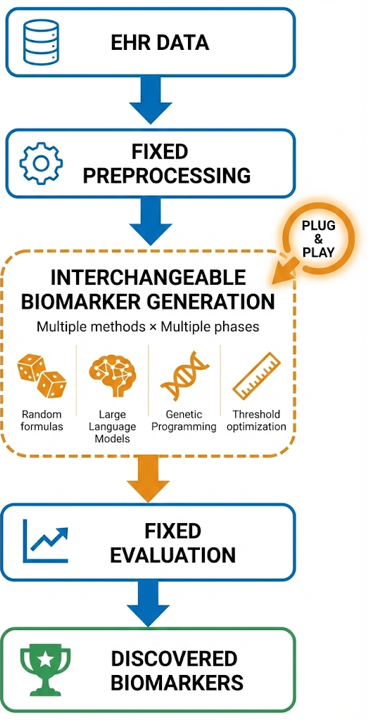
\includegraphics[width=0.43\textwidth]{workflow_diagram.png}
\caption{Agentic framework architecture with interchangeable biomarker generation logic.}
\label{fig:framework}
\vspace{-10pt}
\end{wrapfigure}

This research proposes an agentic framework with interchangeable logic for systematic biomarker discovery from electronic health records. The core innovation lies in separating three distinct components: (1) a fixed data pipeline for preprocessing and validation, (2) interchangeable biomarker generation methods that can be systematically compared, and (3) a standardized evaluation protocol ensuring fair comparison across methods \cite{ref12,ref21}.

The framework enables controlled experimentation by maintaining consistent data inputs and evaluation metrics while varying only the biomarker generation approach. Figure~\ref{fig:framework} illustrates the overall architecture, highlighting the separation between fixed pipeline components and the interchangeable biomarker generation module that enables systematic method comparison.

This design addresses a critical gap in existing literature, where studies apply individual methods in isolation without systematic comparison \cite{ref12,ref14,ref16}. By treating biomarker generation methods as modular components, the framework facilitates rapid prototyping and objective performance assessment across diverse algorithmic approaches.

\subsection{Data Source and Preprocessing}

\subsubsection{MIMIC-IV Database}

We utilize the MIMIC-IV (Medical Information Mart for Intensive Care) database, a freely accessible repository containing de-identified health data from over 70,000 ICU admissions and 500,000 hospital admissions at Beth Israel Deaconess Medical Center \cite{ref11}. The database includes comprehensive laboratory results, diagnostic codes, medications, procedures, and clinical notes spanning 2008-2019. MIMIC-IV's strengths include its scale, longitudinal structure, real-world clinical context, and standardized data quality procedures \cite{ref11}. 

Electronic health records like MIMIC-IV enable automated biomarker discovery at scale, as demonstrated by recent work extracting imaging biomarkers directly from routine CT scans for fracture risk assessment \cite{ref29,ref30}. This validates the feasibility of leveraging existing clinical data for systematic biomarker development without requiring additional data collection.


For this study, we extract CBC measurements from the \texttt{labevents} table and diagnostic information from ICD-9 coded diagnoses in the \texttt{diagnoses\_icd} table. The CBC parameters include: hemoglobin (Hb), hematocrit (Hct), red blood cell count (RBC), white blood cell count (WBC) with differential (neutrophils, lymphocytes, monocytes, eosinophils, basophils), platelet count, mean corpuscular volume (MCV), mean corpuscular hemoglobin (MCH), mean corpuscular hemoglobin concentration (MCHC), and red cell distribution width (RDW).

\subsubsection{Target Condition Definitions}

We demonstrate the framework using four immunological and inflammatory conditions as exemplar use cases:

\begin{itemize}
\item \textbf{Rheumatoid Arthritis}: ICD-9 codes 714.x
\item \textbf{Type 1 Diabetes}: ICD-9 codes 250.x1, 250.x3
\item \textbf{Type 2 Diabetes}: ICD-9 codes 250.x0, 250.x2
\item \textbf{Crohn's Disease}: ICD-9 codes 555.x
\item \textbf{Psoriasis}: ICD-9 code 696.1
\end{itemize}

These conditions were selected as representative examples due to their well-characterized CBC abnormalities documented in clinical literature \cite{ref10,ref14,ref15,ref16}, making them suitable for validating the framework's biomarker discovery capabilities.

\subsubsection{Data Preprocessing Pipeline}

The preprocessing pipeline implements several quality control steps to ensure robust biomarker discovery:

\textbf{Temporal filtering}: We extract CBC measurements within variable lookback windows prior to diagnosis, testing multiple time horizons to assess predictive capability across different pre-diagnostic periods. Lookback windows include: 1 week, 1 month, 3 months, 6 months, 1 year, 2 years, and 5 years. This multi-horizon approach enables investigation of how early biomarker signals emerge before clinical diagnosis and identifies optimal prediction windows for each condition \cite{ref6,ref11}. All measurements are taken before diagnosis to avoid circularity where treatment effects might influence biomarker values.

\textbf{Missing value handling}: Patients with incomplete CBC panels are excluded from analysis to ensure consistent feature availability across subjects. For patients with multiple CBC measurements within the lookback window, we extract multiple aggregate statistics to capture temporal patterns: (1) latest value (most proximal to diagnosis), (2) median value (central tendency across measurements), (3) maximum and minimum values (range of variability), and (4) temporal slope (linear trend over time, when $\geq$2 measurements available). These engineered features enable the framework to leverage longitudinal information beyond single time-point measurements \cite{ref6}.

\textbf{Outlier detection}: Physiologically implausible values are identified using domain-informed range constraints derived from clinical references \cite{ref9} and excluded from analysis. For example, hemoglobin values $<$ 3 g/dL or $>$ 20 g/dL, WBC counts $<$ 1 or $>$ 100 $\times$ $10^9$/L, and platelet counts $<$ 10 or $>$ 1000 $\times$ $10^9$/L are flagged as likely measurement or data entry errors.

\textbf{Normalization}: Normalization strategy will be determined empirically by comparing: (1) z-score standardization within the training set \cite{ref21,ref22}, and (2) domain-informed range normalization using clinically established reference intervals \cite{ref9,ref10}. The latter approach may preserve clinical interpretability by maintaining alignment with familiar scales, while the former ensures algorithmic stability. Both approaches will be evaluated to determine which better facilitates formula generation and model convergence.

\subsubsection{External Validation Dataset}

Subject to data access approval, we plan to validate discovered biomarkers on the EHRSHOT (Electronic Health Record Snapshot) dataset to assess generalizability beyond MIMIC-IV \cite{ref11}. EHRSHOT's different patient population, geographic distribution, and EHR system structure provide rigorous external validation, testing whether biomarkers discovered in the intensive care context generalize to broader clinical settings. This validation strategy addresses a critical limitation in biomarker research, where most studies report only internal validation without testing generalizability to independent populations \cite{ref21,ref23}.

\subsection{Experimental Framework: Three-Phase Design}

The experimental framework proceeds through three sequential phases, each building upon previous insights while testing distinct hypotheses about biomarker generation.

\subsubsection{Phase 1: Baseline Single-Feature Methods}

Phase 1 establishes baseline performance using the most predictive individual CBC parameter, serving as a reference point for evaluating more sophisticated multi-feature approaches.

\textbf{Method 1A - Literature-Based Threshold}: We train a logistic regression model on the training set to identify feature importance through coefficient magnitudes \cite{ref21}. The feature with the highest absolute coefficient is selected as the primary biomarker. We then apply clinical thresholds from established medical literature (e.g., hemoglobin $<$ 12 g/dL for anemia in females, $<$ 13 g/dL in males) to create binary disease predictions \cite{ref9,ref10}.

\textbf{Method 1B - Data-Driven Threshold}: Using the same top-ranked feature from Method 1A, we optimize the decision threshold using the Youden Index (J = max[sensitivity + specificity - 1]) on the training set \cite{ref19,ref27}. The Youden Index was selected based on systematic comparisons demonstrating its robustness across diverse biomarker contexts \cite{ref19}. This method quantifies the performance gain achievable through population-specific threshold optimization compared to generalized clinical guidelines.

\subsubsection{Phase 2: Multi-Feature Formula Generation with Data-Driven Selection}

Phase 2 tests three biomarker generation methods using features selected by machine learning models based solely on predictive performance.

\textbf{Feature Selection}: We employ gradient boosting (XGBoost) to rank CBC parameters by feature importance, selecting the top K features (K $\in$ \{3, 5, 10\}) for formula generation \cite{ref22,ref24}. This data-driven approach identifies features with maximum discriminative power regardless of prior clinical knowledge.

\textbf{Method 2A - Random Formula Generation}: We generate random mathematical combinations of the selected features as a baseline for comparison. The search space includes basic arithmetic operations (+, -, $\times$, $\div$), ratios, logarithmic transforms, and square roots. This method establishes the performance achievable through naive formula construction without optimization or domain knowledge \cite{ref12}.

\textbf{Method 2B - Large Language Model Generation}: We employ medical-domain language models to generate biomarker formulas by leveraging accumulated clinical knowledge encoded during pre-training \cite{ref17,ref21}. Structured prompts provide: (1) selected CBC features with descriptions, (2) target disease pathophysiology, (3) examples of validated composite biomarkers (NLR, FIB-4), and (4) constraints on formula complexity. Retrieval-augmented generation (RAG) grounds formula proposals in authoritative medical literature, reducing hallucination risks \cite{ref18}. Generated formulas undergo validation to ensure mathematical validity and physiological plausibility before evaluation.

\textbf{Method 2C - Genetic Programming}: We implement symbolic regression using genetic programming (DEAP library) to evolve optimized biomarker formulas \cite{ref12,ref13}. The approach maintains a population of candidate formulas, evaluates fitness using AUC on a validation set, and iteratively applies crossover and mutation operations to generate improved formulas. Multi-objective optimization (NSGA-II) balances predictive performance against formula complexity, preventing ``bloat'' while maintaining interpretability \cite{ref12}. Post-evolution simplification reduces formula complexity without sacrificing performance.

\subsubsection{Phase 3: Multi-Feature Formula Generation with Literature-Guided Selection}

Phase 3 repeats the three generation methods from Phase 2, but replaces data-driven feature selection with features identified through systematic literature review of disease-specific pathophysiology \cite{ref14,ref15,ref16,ref25}. This tests whether incorporating domain knowledge during feature selection improves biomarker discovery compared to purely data-driven approaches.

For each target condition, we conduct literature review to identify CBC parameters with documented associations to disease pathogenesis, diagnostic utility, or prognostic value. The same three generation methods (2A, 2B, 2C) are then applied to these literature-selected features, enabling direct comparison against Phase 2's data-driven selection strategy.

\subsection{Evaluation Metrics and Validation Strategy}

\subsubsection{Primary Performance Metrics}

\textbf{Area Under ROC Curve (AUC)}: We employ AUC as the primary metric for overall discrimination ability, as it summarizes performance across all possible decision thresholds and is insensitive to class imbalance \cite{ref21,ref22}.

\textbf{Precision-Recall Analysis}: Given the clinical importance of minimizing false positives, we emphasize high positive predictive value while maintaining acceptable sensitivity. Precision-recall curves and area under precision-recall curve (AUPRC) provide detailed characterization of this trade-off \cite{ref12}.

\textbf{Sensitivity and Specificity}: We report sensitivity and specificity at the optimal Youden Index threshold, along with 95\% confidence intervals computed via bootstrapping \cite{ref19,ref28}.

\subsubsection{Interpretability Quantification}

To explicitly measure the interpretability-performance trade-off, we quantify formula complexity using:

\begin{itemize}
\item \textbf{Number of features}: Count of distinct CBC parameters in the formula
\item \textbf{Number of operations}: Total arithmetic, logarithmic, and other mathematical operations
\item \textbf{Tree depth}: Maximum nesting level for GP-generated formulas
\end{itemize}

Formulas are categorized as ``simple'' (1-2 features, $\leq$3 operations), ``moderate'' (3-5 features, 4-10 operations), or ``complex'' ($>$5 features or $>$10 operations) following established interpretability frameworks \cite{ref12,ref23}.

\subsubsection{Validation Protocol}

\textbf{Cross-Validation}: We employ stratified 5-fold cross-validation to ensure robust performance estimation while preserving class distributions in each fold \cite{ref21,ref22}.

\textbf{Temporal Validation}: Data is split chronologically (80\% earliest admissions for training, 20\% most recent for testing) to assess temporal generalizability and simulate prospective deployment \cite{ref11,ref30}. This approach follows established best practices for EHR-based prediction model validation.

\textbf{Statistical Significance}: Pairwise method comparisons use DeLong's test for AUC differences with Bonferroni correction for multiple comparisons. Bootstrap confidence intervals (1000 iterations) quantify estimation uncertainty \cite{ref19}.

\subsection{Implementation Details}

The framework is implemented in Python 3.10+ using scikit-learn for baseline models and evaluation metrics, XGBoost for feature importance, DEAP for genetic programming, and the Hugging Face Transformers library for LLM integration \cite{ref21,ref22}. Experiments are tracked using MLflow to ensure reproducibility, with fixed random seeds (42) for all stochastic components. Hyperparameter optimization for GP (population size, mutation rate, generations) and XGBoost (learning rate, tree depth) employs Bayesian optimization on validation sets to prevent test set leakage.

\section{Experimental Results}
[To be completed]

\section{Conclusions and Future Work}
[To be completed]

\bibliographystyle{plain}
\bibliography{refrences}

\end{document}